\textit{Nota introduttiva}: Le righe di assorbimento si formano quando uno strato di materia non completamente opaca e non completamente ionizzata viene attraversata da luce (con spettro continuo!) proveniente da una sorgente a temperatura più alta. A causa della non completa opacità, la radiazione non può andare in equilibrio termodinamico con la materia, e quindi l'emissione non è più di corpo nero. Al contrario, i fotoni della sorgente di fondo interagiscono con gli atomi dello strato di materiale solamente alle lunghezze d'onda corrispondenti a particolari differenze di energia, tali da eccitare elettroni legati. Perché un fotone sia assorbito è necessaria la presenza di un numero sufficiente di atomi nel giusto stato di eccitazione.

\subsubsection{L'equazione del trasporto radiativo}

Immaginiamo di avere una radiazione che attraversa un gas, un corpo o qualsiasi altra cosa (potrebbe anche essere il mezzo interstellare). Quali fenomeni possono accadere tra radiazione e materia?

%Immaginiamo di avere una qualche sorgente di radiazione che attraversa un gas, un corpo o qualsiasi altra cosa, cioè immaginiamo di avere una sorgente e un oggetto di cui vogliamo sapere le caratteristiche. L'ipotesi che si fa inizialmente è che questo sia un corpo nero, di cui sappiamo tutto; dopodiché la radiazione di questo corpo attraversa la materia di cui non sappiamo niente e che vogliamo studiare: potrebbe essere il mezzo interstellare o la fotosfera del sole. Quest'ultima possiamo immaginarla come un corpo nero prodotto all'interno del Sole, che viene verso di noi. Questo negli stati più esterni, interagendo con la radiazione, produce dei fenomeni che noi cerchiamo di interpretare in termini di costituenti della materia studiata. Quali sono questi fenomeni che possono accadere tra radiazione e materia?

\begin{figure}[H]
   \centering
   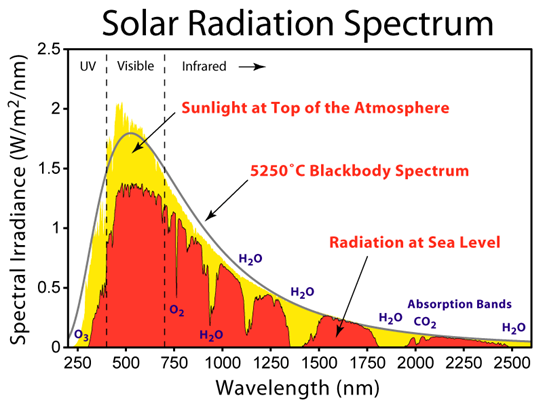
\includegraphics[width=8cm]{immagini/spettro_solare.png}
   %\caption{Spettro radiazione solare}
   %\label{fig:spettro_rad_sol}
\end{figure}

Consideriamo il Sole. Quali sono quei fenomeni che trasformano la curva di un corpo nero (linea continua nera) nello spettro reale solare (colorato in figura di rosso)?

L'obiettivo di questa sezione è quindi quello di interpretare le differenze tra lo spettro del corpo nero e quello della radiazione solare, per capire i materiali da cui è composto il Sole.

Questo processo è molto simile alla tomografia. In quel caso si fa passare una radiazione nota attraverso un corpo e dalle cadute di potenziale si cerca di capire quale sia la sua composizione (questa ad esempio è usata in medicina per capire la distribuzione interna degli organi).

L'astrofisica è la scienza dell'inversione del dato: da una grandezza misurata cerchiamo di ricavare altro, ad esempio dalla magnitudine apparente cerchiamo di ricavare quella assoluta. Per fare questo abbiamo introdotto l'intensità specifica, che ricordiamo essere quella quantità che definisce la perdita di energia quando un pennello di radiazione attraversa una superficie $dS$, proiettata in un angolo $\theta$, all'interno di un cono $d\omega$ per unità di frequenza e per unità di tempo. Questa è la quantità che vogliamo valutare. Abbiamo appena visto che la radiazione, attraversando la materia, ha una attenuazione che genericamente possiamo dire essere dovuta a scattering.

Immaginiamo un atomo all'interno dell'assorbitore (ossia il materiale attraversato), possiamo immaginare che in questo caso l'energia per esempio è stata catturata da un elettrone della shell k\footnote{I livelli orbitali negli atomi sono indicati con lettere. Quella più interna si chiama k. I fotoni X vengono tutti dalla shell k.}. Se un fotone molto energetico colpisce un atomo può estrarre un elettrone, con conseguente perdita di energia. Di questa tipologia di eventi ne succedono tantissimi. Solitamente gli astrofisici li raggruppano per frequenza, non importa se ad assorbire questa frequenza è stato l'elettrone nella shell k dell'atomo del ferro o del potassio (che in questa fase non sappiamo distinguere). Infatti quello che vediamo è una diminuzione di energia, che viene espressa, come già visto, con il coefficiente di assorbimento.

Concentriamoci adesso su questo processo d'urto. Immaginiamo di avere un fotone che colpisce un atomo con una certa sezione d'urto\footnote{È quella superficie geometrica per cui si ha una interazione.}.

Quando si parla di trasporto radiativo si fa riferimento al numero di assorbitori (che ad esempio potrebbero essere gli atomi o molecole). In questo caso rappresentiamo la perdita di intensità in termini di un coefficiente detto \textbf{coefficiente di estinzione} o \textbf{opacità}.

Se abbiamo un fotone, il percorso che esso può compiere nel mezzo è proprio il reciproco del coefficiente di estinzione. Questo perché il coefficiente di estinzione rappresenta, in qualche modo, una probabilità di interazione e quindi il suo reciproco è il percorso del fotone nel mezzo. Questo viene solitamente chiamato libero cammino medio. Vi è una relazione tra il coefficiente di assorbimento ($k_\nu$) e quello di opacità ($\chi_\nu$):

\begin{equation}
  k_\nu = \frac{\chi_\nu}{\rho}
\end{equation}

dove $\rho$ è la densità del mezzo.

Immaginiamo di avere un certo numero di particelle all'interno di un volume e di avere un fotone che attraversa tale volume. La probabilità che il fotone urti ognuna delle particelle dipende dalla sezione d'urto delle particelle, ad esempio se la particella è grande quanto la superficie presa in considerazione, sicuramente il fotone la colpisce. Il fatto che la sezione d'urto sia più piccola, dà al fotone la possibilità di attraversarla senza urtare. Questa sezione d'urto si deve però relazionare al numero di particelle: se abbiamo piccole sezioni d'urto ma tantissime particelle da creare un muro, il fotone non passa lo stesso. Se supponiamo che la sezione d'urto sia molto più piccola del quadrato della distanza media tra le particelle, la probabilità andrebbe come $n^{-\frac{1}{3}}$ con $n$ numero di particelle\footnote{In realtà dimensionalmente dovrebbe essere una densità di particelle.}.

Quindi l'ipotesi fatta permette di associare la perdita di energia del fotone al numero di particelle stesso (cosa che sennò non potremmo fare perché ad esempio possiamo avere una particella che fa ombra alle altre e quindi in questo caso la probabilità di interazione non sarebbe più legata al numero di particelle, perché le particelle in ombra non hanno possibilità di interagire). Quello che dunque accade è che il coefficiente di estinzione è proporzionale al prodotto del numero di particelle\footnote{Sempre per farlo quadrare dimensionalmente dovrebbe essere una densità di particelle.} per la loro sezione d'urto. Questo è molto utile perché ci permette di determinare la numerosità delle particelle, che in astrofisica è detta \textit{abbondanza}. 

Nei discorsi precedenti abbiamo implicitamente assunto che le particelle fossero sferiche. Infatti se così non fosse, ad esempio se avessero una forma allungata, dovremmo considerare pure l'orientazione delle particelle. Questa ipotesi conferisce quindi un'isotropia al nostro sistema, e ciò rende non necessaria la direzione da cui arriva la radiazione (che altrimenti dovremmo sapere). Un esempio di mezzo non isotropo è il mezzo interstellare, il quale è costituito da grani aventi forma allungata che normalmente si allineano con il campo magnetico intergalattico. Il problema diventa decisamente più complicato perché per risolverlo dobbiamo conoscere l'orientamento nello spazio.

Un'altra ipotesi che abbiamo fatto è che l'oggetto sia fermo, infatti in caso contrario esso percepirebbe la frequenza del fotone in maniera diversa (rispetto a quella del sistema di riferimento in cui il fotone è fermo) per effetto Doppler, quindi per far scappare l'elettrone dall'atomo abbiamo bisogno di un fotone di frequenza diversa, per cui il coefficiente di assorbimento dipenderebbe anche dalla velocità. In altre parole, ci siamo messi in condizioni semplificate in cui il mezzo è fermo e isotropo, e in questo caso l'equazione è quella trovata prima.

Un altro possibile processo che si può avere e che non possiamo escludere è che il mezzo aggiunga fotoni, per cui la radiazione uscente risulterà più intensa rispetto a quella entrante. Allora nel discutere di come la radiazione si trasferisce in un mezzo, oltre gli effetti di assorbimento dobbiamo anche valutare gli effetti di introduzione di radiazione nella direzione di osservazione, perché quello che doveva essere un mezzo inerte è in realtà esso stesso una sorgente.

Immaginiamo che esista un coefficiente macroscopico, che indichiamo con $\eta$, che è capace di rilasciare una certa quantità di energia nella direzione in cui stiamo osservando. Quindi noi di fatto diciamo che questo aumento di intensità si possa imputare completamente a questo macro-parametro, chiamato \textbf{emissività} o \textbf{coefficiente di emissione}\footnote{Questo coefficiente in realtà possiamo pensarlo come l'aumento di intensità che si ha quando la radiazione attraversa un tratto di materia completamente emettente. Di fatto serve a quantificare la variazione di energia della radiazione.}. Questo parametro può avere una forte dipendenza dalla frequenza, ma questo non è sempre detto. %Il minimo che ci possiamo aspettare è che sia come un corpo nero.

In generale la materia emette e assorbe e l'equazione che regola la variazione di intensità di una radiazione che attraversa un tratto $ds$ è:

\begin{equation}
  \frac{dI_{\nu}}{ds} = \eta_{\nu} - \chi_{\nu} I_{\nu}
  \label{eq:trasp_rad}
\end{equation}

detta \textbf{equazione del trasporto radiativo}, ed è una delle equazioni più importanti per gli astrofisici. Di solito anziché usare il coefficiente di emissività si preferisce introdurre la funzione sorgente $S_{\nu}$

\begin{equation}
  S_{\nu}=\frac{\eta_{\nu}}{\chi_{\nu}}
\end{equation}

e l'equazione precedente diventa:

\begin{equation}
  \frac{dI_{\nu}}{ds}=\chi_{\nu} \left( S_{\nu} - I_{\nu} \right)
\end{equation}

Che può essere risolta numericamente.

Ricapitolando, l'idea è osservare cosa accade alla radiazione attraversando la materia, cioè vogliamo studiare in che modo si modifica la radiazione di ingresso. Per poterla descrivere abbiamo introdotto un coefficiente di assorbimento e un coefficiente di emissione. Potremmo quindi dire che, per ogni elemento di materia di spessore $ds$, la radiazione in ingresso viene modificata di una certa quantità dovuta ad una perdita per assorbimento e ad una emissione della materia.

Per noi è importante capire quali siano i processi responsabili della modifica della radiazione. Soffermiamoci su questo aspetto prima di risolvere numericamente l'equazione.
\subsubsection{Processi che modificano la radiazione}
Classicamente suddividiamo le possibili interazioni radiazione-materia in tre categorie:

\begin{enumerate}
    \item Processo di \textbf{vero assorbimento} del fotone: un fotone incide, in qualche modo interagisce con la materia e scompare. Questo non vuol dire che l'energia del fotone si è persa, semplicemente è stata convertita da energia del campo di radiazione in energia cinetica della materia. L'energia quindi permane ma scompare un fotone, ovvero quella particella che nel nostro spettrografo avrebbe dato nel conteggio un valore.
    \item Processo di \textbf{vera emissione}: i fotoni che osserviamo vengono effettivamente generati nella materia. \E quindi possibile generare energia nella materia e convertirla in radiazione.
    \item Processo di \textbf{scattering}: se un fotone si sta propagando verso di noi e viene deviato dal suo percorso per noi non è più misurabile, però il fotone non è scomparso. La differenza rispetto ai processi precedenti è che nello scattering non c'è nessuna variazione di energia all'interno del sistema, semplicemente il fotone è stato deviato, ma la quantità di energia non cambia (non si è passati, ad esempio, da energia cinetica ad energia del campo di radiazione).
\end{enumerate}

\comment{\begin{figure}[H]
   \centering
   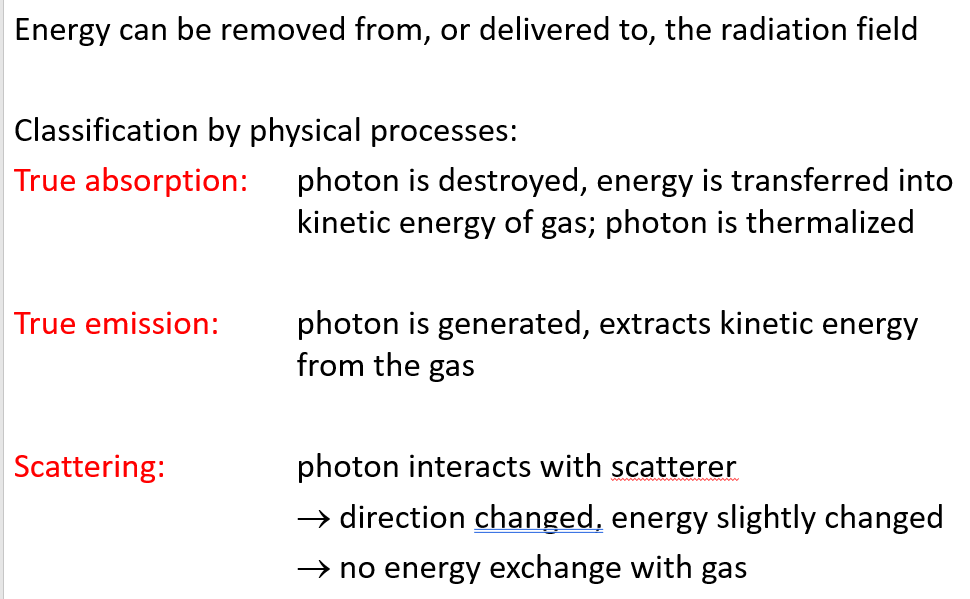
\includegraphics[width=7cm]{28-10.1(interazione_radiazione-materia).png}
    %\caption{Interazioni radiazione-materia}
   \label{fig:28-10.1(interazione_radiazione-materia)}
\end{figure}}

$\bullet$ \textbf{Vero assorbimento}
Vediamo ora quali sono i processi che possono portare ad un vero assorbimento.

I fotoni hanno una certa quantità di energia $h\nu$. Se questa quantità è sufficiente a ionizzare un atomo, il risultato è che il fotone scompare e compare energia cinetica in termini di un elettrone che si sta muovendo, quindi ci sarà una particella in più nel nostro gas (che poi sostanzialmente è un plasma) e che ha una velocità tale che

$$\frac{1}{2}m_{e}v^{2}=E-E_{in}$$

con $E$ energia iniziale del fotone e $E_{in}$ energia di ionizzazione. Da questa relazione risulta chiaro che l'elettrone avrà una velocità minore del fotone, ciò significa che la velocità di questo elettrone non è immediatamente legata all'energia del fotone, ma è connessa all'energia di ionizzazione (può essere che ne serva poca, può essere che ne serva tanta). A parità di $E$, in un caso come quello di ionizzazione dell'orbitale più interno, l'energia necessaria per l'estrazione dell'elettrone è altissima, quindi gli elettroni che vengono fuori sono lenti; se invece eseguiamo la ionizzazione su un orbitale più esterno, gli elettroni possono essere velocissimi.

Questo è un punto fondamentale di tutto il discorso: noi possiamo trasferire energia dalla radiazione al plasma in termini di energia cinetica. Aumentare l'energia cinetica di un plasma significa aumentarne la temperatura, e lo spetto di corpo nero emesso da un corpo dipende dalla sua temperatura ed è descritto dalla \textbf{funzione di Planck}.

\begin{figure}[H]
   \centering
   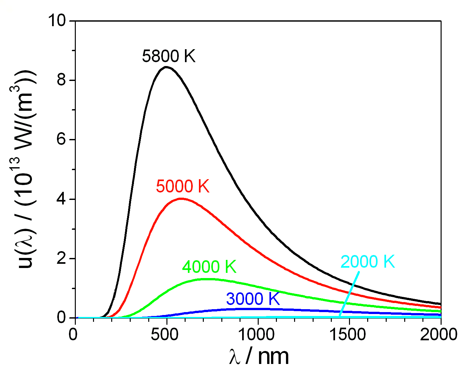
\includegraphics[width=8cm]{28-10.4(funzione di Planck).png}
   \label{fig:28-10.4funzione di Planck}
\end{figure}

Dunque stiamo trasferendo l'energia di fotoni di frequenza ben precisa alla materia, la quale restituirà un nuovo spettro. 
%Quindi il processo non è neanche semplice da prevedere in quanto, l'energia assorbita dal singolo fotone, in termini di energia cinetica, restituisce un altro campo di fotoni.
%La questione è complicata perché quello che alla fine vogliamo fare è risolvere l'equazione del trasporto radiativo mettendo dentro i coefficienti di assorbimento e di emissione, ma le due cose possono essere legate, nel senso che se i fotoni vengono assorbiti in volumi piccoli si può avere un equilibrio, se i fotoni invece lasciano la materia allora possiamo avere il raffreddamento del gas stesso.

Si parla quindi di assorbimento in termini della radiazione che noi osserviamo. Pensiamo ad esempio al Sole: il suo spettro è il prodotto dei fotoni assorbiti, fotoni che sono stati prodotti nelle zone più interne del Sole e poi sono stati assorbiti dalla fotosfera e lì processati con una serie di assorbimenti, per poi restituire una curva dalla forma completamente diversa rispetto alla curva della planckiana prodotta all'interno del Sole.

\vspace{0.2cm}$\bullet$ \textbf{Vera emissione}

Abbiamo detto che possiamo effettivamente trasferire energia dalla radiazione al gas in forma di energia cinetica, possiamo però fare anche il contrario: possiamo produrre fotoni estraendo l'energia cinetica del gas. Ciò accade sostanzialmente con urti.

Immaginiamo di avere due atomi di idrogeno con gli elettroni nell'orbitale più basso. Tali atomi non sono però da soli, si muovono e collidono; nella collisione può accadere che uno dei due atomi porti l'elettrone dal livello più basso a quello più alto:

\begin{figure}[H]
    \centering
    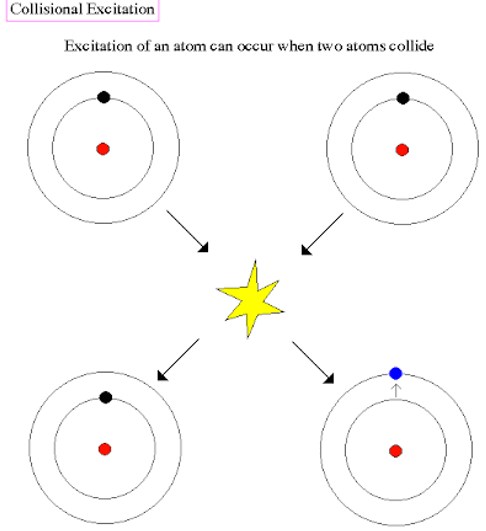
\includegraphics [width=7cm]{28-10.6(eccitazione_per_collisione).png}
    \label{fig:eccitazione_per_collisione}
\end{figure}

Quando immaginiamo questo processo, non dobbiamo visualizzarlo come se fosse un semplice urto tra due biglie, perché non è questo quello che avviene nella realtà. Questi orbitali sono quelli ricavati dalla soluzione analitica dell'equazione di Schrödinger nel caso di un elettrone con un protone, ma quando abbiamo due atomi l'elettrone risentirà sì del campo elettrico del protone, ma vedrà anche il campo elettrico dell'elettrone dell'atomo accanto oppure vedrà il campo elettrico del protone accanto. Quello che succede in questi casi è che si modifica totalmente l'orbitale, e l'elettrone, spazialmente, si collocherà in un altro luogo. Passato il perturbatore, l'elettrone si ritroverà nella configurazione precedente (quella prima della perturbazione), dove il luogo che sta occupando non sarà più l'orbitale per $n=1$, ma l'orbitale per $n=2$. L'atomo dunque si ritrova in uno stato eccitato, ma quando l'elettrone si trova nell'orbitale più elevato, decade naturalmente (l'elettrone non può stare in questo stato eccitato) producendo un fotone.

In definitiva, dall'energia cinetica per collisione di atomi possiamo creare una radiazione.

Questo processo è più complicato da prevedere, perché il fotone che viene emesso avrà frequenza dipendente dagli atomi che stiamo considerando. Nel caso di atomi di idrogeno la transizione sarebbe la Lyman alpha (1216 Å), nel caso di un atomo di elio ci sarebbe un'altra frequenza. Quindi bisogna fare un calcolo puntuale mettendo dentro tutta la composizione chimica degli agenti che si vogliono fare interagire con il campo di radiazione.

\vspace{0.2cm}$\bullet$ \textbf{Scattering}

\vspace{0.2cm}Lo scattering è sostanzialmente \textit{l'assorbimento e la riemissione della stessa frequenza, però lungo direzioni diverse}, ossia l'elettrone vede il campo elettrico del fotone, oscilla con quella frequenza e poi lo riemette in un'altra qualunque direzione (non c'è una direzione privilegiata, può essere anche all'indietro).

Per la precisione il fotone viene riemesso con la stessa frequenza solo se supponiamo che la materia sia ferma. In questo caso si parla di \textbf{scattering Thomson} (abbiamo un elettrone da qualche parte, esso vede il campo elettrico, oscilla e riemette totalmente; è una riemissione identica a quella iniziale, quindi di fatto non modifichiamo l'energia del sistema).

Nella realtà gli atomi di idrogeno sono ovviamente in un gas con velocità media. La conseguenza di tale effetto è che quando un elettrone all'interno dell'atomo assorbe un fotone di frequenza $\nu_1$ e passa allo stato eccitato, quando decade emetterà un fotone la cui frequenza sarà pari a $\nu_2$, diversa dalla prima a causa dell'effetto Doppler. In particolare si ha:

\begin{equation}
  \Delta\lambda=\lambda \left(1 + \frac{VR}{c}\right)
\end{equation}

Dunque, nel processo di scattering si ha semplicemente una perdita dell'energia della radiazione, per il gas non è cambiato niente.

Quando si parla di scattering con un atomo possiamo avere variazione della $\lambda$ emessa dal fotone oppure la diffusione di fotoni su elettroni liberi. Se invece gli elettroni sono liberi si parla di \textbf{scattering Thomson} (abbiamo un elettrone da qualche parte, esso vede il campo elettrico, oscilla e riemette totalmente; è una riemissione identica a quella iniziale, quindi di fatto non si modifica l'energia del sistema).

\vspace{0.2cm}Ci possono però essere strane situazioni intermedie un atomo.

Supponiamo di avere un atomo con un elettrone sul livello A, che passa ad un livello C perché assorbe un fotone. Dal livello C il fotone può ritornare al livello A, ma potrebbe anche andare su un livello intermedio B e poi da quest'ultimo tornare ad A. In questo caso dall'assorbimento di un fotone se ne sono prodotti due (nota: l'energia è comunque la stessa). Nel caso dell'idrogeno, esso potrebbe ad esempio assorbire un fotone di lunghezza 4100 \AA e tirarne fuori uno di 4800 \AA e uno di 6500 \AA, passando cioè da un H-$\gamma$ ad un H-$\beta$ e un H-$\alpha$ e quindi immettiamo nel campo di radiazione fotoni che prima non esistevano. Questo processo di decadimento è chiamato \textbf{fluorescenza}.

%Tutto questo si può effettivamente mischiare in una maniera complicata immaginando che uno possa avere transizioni da un livello ad un altro per urti, che poi riemettono fotoni e robe di questo genere.Il bilancio non è semplicissimo: dati tutti questi processi noi dovremmo inserirli nell'equazione del trasporto come coefficienti di emissione e di assorbimento.

\subsubsection{Risoluzione dell'equazione del trasporto radiativo}

Ricordiamo l'equazione del trasporto radiativo:

$$\frac{dI_{\nu}}{ds}=\chi_{\nu}(S_{\nu}-I_{\nu})$$

In linea di principio, tale equazione dovrebbe essere risolta in coordinate sferiche, ma possiamo operare un'approssimazione: il raggio della superficie di emissione (fotosfera\footnote{Regione che emette luce e in corrispondenza della quale esso diventa opaco.}) è molto più piccolo del raggio della stella stessa, per cui possiamo immaginare che l'atmosfera di un oggetto sia rappresentabile come strati piani e paralleli.
% in questo modo la direzione sulla direzione perpendicolare sarà uguale alla direzione di osservazione

%Se invece fate questa cosa tenendo conto della curvatura, dovrete risolverla in due direzioni diverse.

\begin{figure}[H]
    \centering
    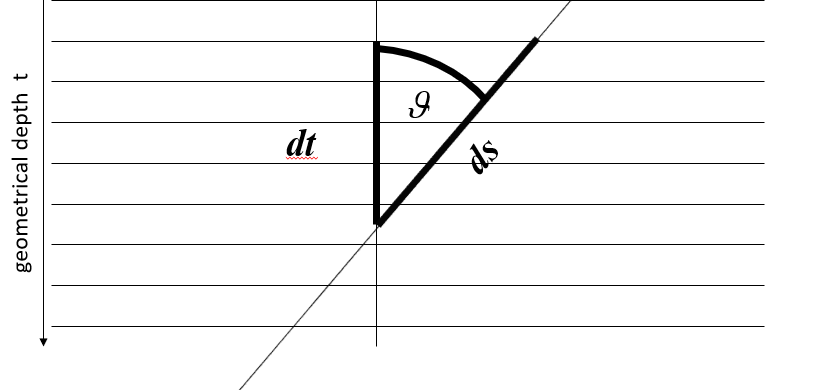
\includegraphics[width=7cm]{28-10-15(geometria_risoluzione_equazione_trasporto_radiativo).png}
    \label{fig:geometria_eq_trasporto_radiativo}
\end{figure}

Supponiamo che la direzione di osservazione formi un angolo $\vartheta$ con la normale a tali strati, la sua proiezione su quest'ultima sarà pari a $dt=-\mu ds$ dove $\mu=\cos\theta$. Segue che

$$\frac{dI_{\nu}}{ds}=-\mu\frac{dI_{\nu}}{dt}$$

e l'equazione potrà scriversi come

\begin{equation}
  -\mu\frac{dI_{\nu}}{dt}=\chi_{\nu}(S_{\nu}-I_{\nu})
\end{equation}

Introduciamo, in luogo della coordinata geometrica $s$, la cosiddetta profondità ottica specifica (funzione di $\nu$), attraverso l'equazione

$$d \tau_{\nu}=-\chi_{\nu} \, ds$$

Come mostra l'equazione, la profondità ottica è definita in direzione opposta a quella di propagazione della radiazione, il che riflette il punto di vista di un osservatore che riceve la radiazione nel proprio strumento (vedi figura sotto). Vedremo che useremo questo punto di vista, cioè poi andremo a integrare dall'esterno verso l'interno. Vediamo perché.

Noi abbiamo una certa quantità di radiazione che incide sul nostro gas e questa ovviamente si estinguerà, poi all'interno del gas dobbiamo sommare i contributi dell'intensità che vengono fuori dalla funzione sorgente. Una volta che lo abbiamo calcolato, dobbiamo chiederci di quanto si è estinto questo contributo. Se facciamo il calcolo dall'esterno possiamo andare dentro fino a quando non scopriamo che il contributo viene totalmente estinto ed in quel momento finiamo l'integrazione (smettiamo di portare avanti il calcolo). Con l'idea che la materia abbia una densità che aumenta dall'esterno verso l'interno, è ragionevole pensare che all'interno $\tau_{\nu}$ sia infinito, ma siccome l'integrale lo risolviamo numericamente, nella pratica raggiunto un certo valore di $\tau_{\nu}$ tronchiamo l'integrazione, quindi risolviamo tutto in maniera più rapida piuttosto che risolvere l'integrale al contrario, perché in quel caso calcolando la funzione sorgente scopriremmo che la quantità di spazio è talmente grande che tutti i fotoni vengono assorbiti. Questa semplificazione pratica nasce anche dall'osservazione che in astrofisica, quando si parla di trasporto radiativo, in qualche modo si immagina che le sorgenti siano di infinite dimensioni, pertanto la materia viene totalmente estinta. Nel caso del Sole e della fotosfera (l'atmosfera solare), i fotoni provengono dall'interno (ancora non ne sappiamo la ragione) e attraversano quest'ultima, la quale è profonda 500 km (spazio estremamente piccolo rispetto alle dimensioni della stella). Quello che si può immaginare è che $\tau_{\nu}$, in questo piccolo spazio, arrivi ad essere infinito. Quindi quello che era in realtà il flusso prodotto all'interno viene posto uguale a 0 e l'intensità emergente sarà data soltanto dal contributo della funzione sorgente in ogni strato, consideratala la sua estinzione in quella successiva.

\begin{figure}[H]
  \centering
  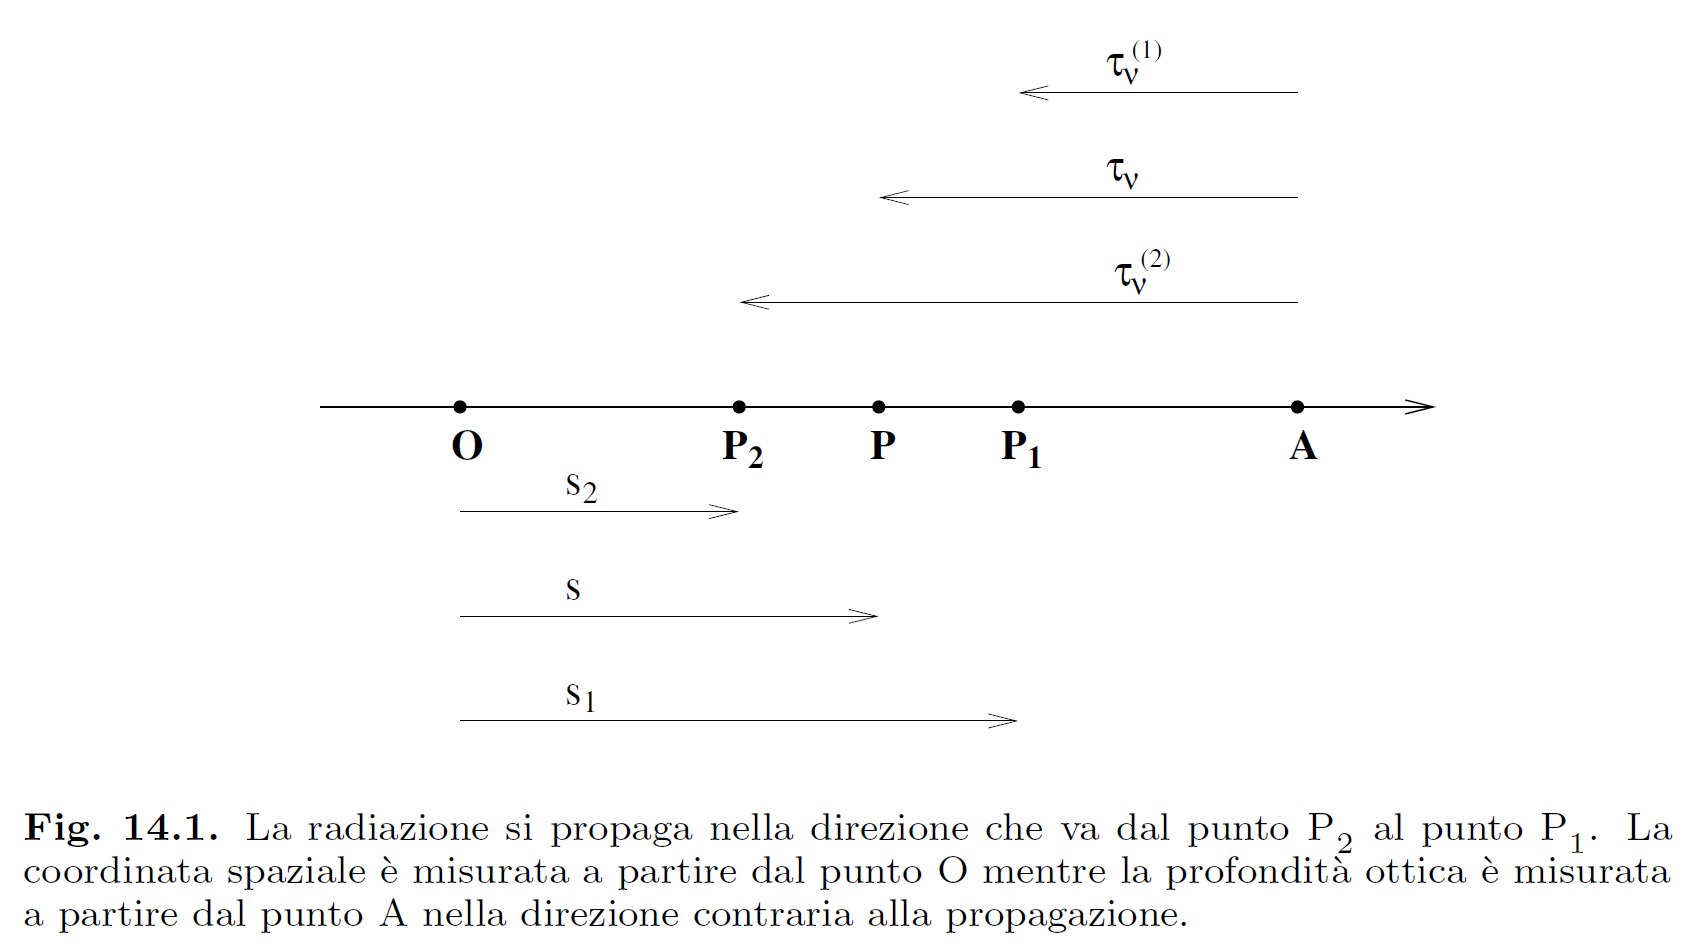
\includegraphics[width=14cm]{immagini/direzione_risoluzione_eq_trasporto_radiativo.png}
\end{figure}

Considerando il plasma contenuto entro uno spessore geometrico fissato, ad esempio fra i punti $P_1$ e $P_2$ della figura seguente, caratterizzati dalle coordinate $s_1$ e $s_2$ (con $s_1>s_2$), lo spessore ottico risulta, per semplice integrazione dell'equazione precedente

\begin{equation}
  \tau_{\nu}(P_1,P_2)=\int_{s_2}^{s_1} \chi_{\nu}(s) \, ds
\end{equation}

Lo spessore ottico dipende dalla frequenza e uno spessore geometrico fissato si definisce \textit{otticamente sottile} quando $\tau_{\nu} \ll 1$ oppure \textit{otticamente spesso} quando $\tau_{\nu} \gg 1$. In termini fisici, un mezzo è otticamente sottile alla frequenza $\nu$ quando un fotone di quella frequenza ha una probabilità trascurabile di essere assorbito nell'attraversarlo. Viceversa, se il mezzo è otticamente spesso, il fotone ha una probabilità praticamente uguale a uno di essere assorbito nel mezzo stesso.

\vspace{0.2cm}Mettiamoci nel caso semplificato in cui $\mu=1$, quindi $ds=-dt$. Dividendo l'equazione del trasporto per $\chi_{\nu}$ e cambiando di segno, si ottiene

\begin{equation}
  \frac{dI_{\nu}}{d \tau_{\nu}}=I_{\nu} - S_{\nu}
\end{equation}

Per risolvere questa equazione moltiplichiamo ambo i membri per il fattore $e^{-\tau_{\nu}}$ . Si ottiene

$$e^{-\tau_{\nu}} \frac{dI_{\nu}}{d \tau_{\nu}}
=e^{-\tau_{\nu}} I_{\nu} - e^{-\tau_{\nu}} S_{\nu}$$

ovvero\footnote{In questo passaggio è stata usata la relazione
$$e^{-\tau_\nu}\frac{dI_{\nu}}{d\tau_{\nu}} - e^{-\tau_\nu}I_{\nu}=\frac{d}{d \tau_{\nu}} \big( e^{-\tau_\nu} I_{\nu} \big)$$
dovuta alla regola di derivazione del prodotto.}

\begin{equation}
  \frac{d}{d \tau_{\nu}} \left( e^{-\tau_{\nu}}I_{\nu} \right)=-e^{-\tau_{\nu}} S_{\nu}
\end{equation}

Quello che succede è che i fotoni entrano nell'atmosfera, vengono estinti esponenzialmente attraversando uno strato, ma quest'ultimo emetterà qualcosa che verrà anch'esso estinto esponenzialmente (e ciò avviene in ogni strato).

Facendo riferimento alla figura sopra, integriamo questa equazione fra i punti $P_2$ e $P_1$ del cammino percorso dal raggio ai quali corrispondono le profondità ottiche $\tau_{\nu}^{(2)}$ e $\tau_{\nu}^{(1)}$ con $\tau_{\nu}^{(1)}<\tau_{\nu}^{(2)}$. Si ottiene

$$e^{-\tau_{\nu}^{(1)}} I_{\nu} \left( \tau_{\nu}^{(1)} \right) - e^{-\tau_{\nu}^{(2)}} I_{\nu} \left( \tau_{\nu}^{(2)} \right)
=-\int_{\tau_{\nu}^{(2)}}^{\tau_{\nu}^{(1)}} S_{\nu}(\tau_{\nu}) e^{-\tau_{\nu}} \, d\tau_{\nu}$$

ovvero

$$I_{\nu} \left( \tau_{\nu}^{(1)} \right)
=I_{\nu} \left( \tau_{\nu}^{(2)} \right) e^{-\left( \tau_{\nu}^{(2)} - \tau_{\nu}^{(1)} \right)} + \int_{\tau_{\nu}^{(1)}}^{\tau_{\nu}^{(2)}} S_{\nu}(\tau_{\nu}) e^{- \left( \tau_{\nu} - \tau_{\nu}^{(1)} \right) } \, d\tau_{\nu}$$

Nota: abbiamo invertito gli estremi dell'integrale, quindi come accennato poc'anzi adesso stiamo integrando dall'esterno verso l'interno.

Questo risultato si interpreta facilmente osservando che l'intensità nel punto $P_1$ è data dall'intensità presente nel punto $P_2$ (la condizione al contorno) moltiplicata per il fattore di attenuazione dovuto all'assorbimento fra i punti $P_2$ e $P_1$, alla quale si aggiunge il contributo dovuto all'emissione nell'intervallo compreso fra i due punti. Il contributo relativo all'intervallo infinitesimo $d\tau_{\nu}$, situato nell'intorno del punto generico $P$, è moltiplicato per il relativo fattore di attenuazione dovuto all'assorbimento fra i punti $P$ e $P_1$. In particolare, se si considera la radiazione emergente da un plasma e si pone quindi $\tau_{\nu}^{(1)}=0$, l'equazione precedente si può anche porre nella forma

\begin{equation}
  I_{\nu}(0)=I_{\nu}(\tau_{\nu}) e^{-\tau_{\nu}} + \int_{0}^{\tau_{\nu}} S_{\nu}(\tau'_{\nu}) e^{-\tau'_{\nu}} d\tau'_{\nu}
  \label{eq:sol_trasp_rad}
\end{equation}

In molti casi, soprattutto in astrofisica, si ha a che fare con plasmi che risultano praticamente infiniti in una direzione (si pensi ad esempio a un'atmosfera stellare della quale interessi esprimere l'intensità emergente in funzione delle proprietà locali dell'atmosfera stessa). In tali casi, si deve considerare il limite dell'equazione precedente per $\tau_{\nu} \to \infty$ e, supponendo matematicamente che si abbia

$$\lim_{\tau_{\nu} \to \infty} I_{\nu}(\tau_{\nu}) e^{-\tau_{\nu}}=0$$

si ottiene

\begin{equation}
  I_{\nu}(0)= \int_{0}^{\infty} S_{\nu}(\tau_{\nu}) e^{-\tau_{\nu}} d\tau_{\nu}
  \label{eq:sol_trasp_rad_spessore_infinito}
\end{equation}

Il limite matematico di cui sopra è sempre soddisfatto in pratica perché, nel caso opposto, si troverebbe il risultato assurdo che l'intensità emergente dal mezzo assume un valore infinito. L'equazione esprime in tutta generalità l'intensità emergente da un mezzo semi-infinito, ovvero da un mezzo indefinito nella direzione opposta a quella sotto la quale si riceve la radiazione. Essa è alla base dell'interpretazione quantitativa degli spettri stellari.




%Quello che succede è che l'intensità emergente è quella in ingresso, estinta per l'intero $\tau$, più quello che viene prodotto in ognuno degli strati estinto da quel punto alla fine (quest'ultimo è il significato dell'integrale numerico).

%Questa soluzione funziona, per calcolare l'integrale ho bisogno di $\tau$ come ingrediente (ovviamente dobbiamo avere idea di cosa è entrato).

Prima di proseguire, torniamo alla \eqref{eq:sol_trasp_rad} e distinguiamo due casi in basi al valore di $\tau_{\nu}$:

\begin{itemize}
  \item Nel caso di mezzo otticamente sottile, ossia per $\tau_{\nu} \ll 1$ (quindi $e^{-\tau_{\nu}} \approx 1$), un fotone di frequenza $\nu$ ha una probabilità quasi nulla di essere assorbito. La radiazione emergente dal plasma sarà allora
  \begin{equation*}
    I_{\nu}(0)=I_{\nu}(\tau_{\nu}) + \int_{0}^{\tau_{\nu}} S_{\nu}(\tau'_{\nu}) \, d\tau'_{\nu}
  \end{equation*}
  \item Nel caso di mezzo otticamente spesso, ossia per $\tau_{\nu} \gg 1$ (quindi $e^{-\tau_{\nu}} \approx 0$), un fotone di frequenza $\nu$ ha probabilità quasi uguale a 1 di essere assorbito. La radiazione emergente dal plasma sarà allora
  \begin{equation*}
    I_{\nu}(0)=\int_{0}^{\tau_{\nu}} S_{\nu}(\tau'_{\nu}) e^{-\tau'_{\nu}} \, d\tau'_{\nu}
  \end{equation*}
\end{itemize}

\E chiaro che per risolvere l'integrale dobbiamo conoscere $\tau_\nu$ e quindi $\chi_\nu$; inoltre dovremo determinare la funzione sorgente. Quello che si fa nella pratica per la risoluzione è campionarlo (non possiamo fare l'integrale per tutte le frequenze, dobbiamo fare un campionamento).
%Siccome stiamo parlando di qualcosa che potrebbe essere l'atmosfera terrestre, questo è vero per ognuno degli strati dove magari la densità atmosferica non cambia (ogni strato avrà comunque un'estinzione che dipenderà dal numero di particelle, le proprietà ottiche magari sono uguali, però le particelle stanno cambiando di numero).

Si potrebbe immaginare che l'intensità emergente sia la media pesata della funzione sorgente lungo la linea di vista. Cioè, se ogni strato viene estinto, di fatto è come se facessimo la somma dei contributi con un peso (e matematicamente questa è la trasformata di Laplace).

%\vspace{0.2cm}Vediamo cosa succede nel caso in cui $\tau \gg 1$, ossia nel caso in cui l'estinzione diventa tale da non far emergere più niente: la materia è così densa che la radiazione non riesce ad attraversarla.

%Nota: questo non è vero per tutte le singole lunghezze d'onda. La materia può infatti essere totalmente opaca ad una lunghezza d'onda e trasparente ad altre (ricordando il lavoro di Fraunhofer, il Sole nelle strisce nere ha $\tau$ infinito, fuori dalle bande il $\tau$ può essere zero e quindi la radiazione può emergere).

\vspace{0.2cm}Confrontiamo ora il risultato di questa integrazione con gli spettri osservati. Rappresentiamo di seguito la luminosità della stella in funzione della lunghezza d'onda:

\begin{figure}[H]
    \centering
    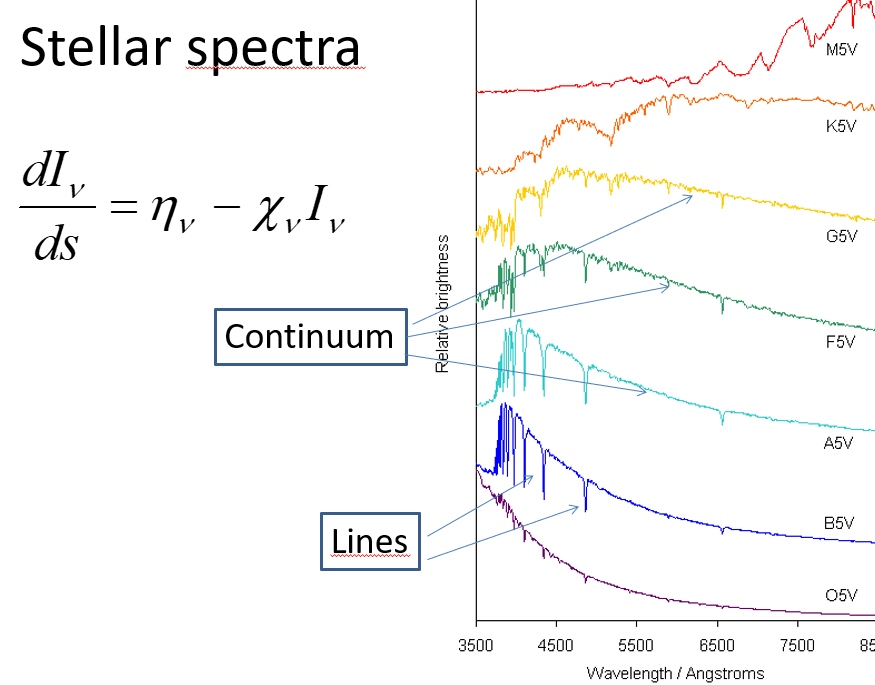
\includegraphics[width=9cm]{28-10.20(spettri_stellari).png}
    \label{fig:spettri stellari}
\end{figure}

Negli spettri stellari (grafici dell'energia in funzione della lunghezza d'onda), che possono avere tra loro forma molto diversa, si è osservata una chiara distinzione di comportamento della distribuzione spettrale con la lunghezza d'onda in due grandi categorie:

\begin{itemize}
    \item Una parte definita \textbf{continuo}, che cambia poco con la lunghezza d'onda;
    \item Le \textbf{righe spettrali}, strutture che variano molto rapidamente con la lunghezza d'onda: sono le bande nere dello spettro di Fraunhofer\footnote{Fraunhofer realizzò che lo spettro colorato del Sole presentava delle righe nere.}.
\end{itemize}

La teoria ci dice che la radiazione si trasmette attraverso la materia con un'interazione che noi possiamo quantificare parlando di coefficienti di estinzione e di emissione. Ci chiediamo a questo punto se siamo in grado di invertire lo spettro osservato che è il risultato dell'equazione del trasporto per estrarre l'estinzione e l'emissione. Il problema dell'astrofisica è proprio questo: possiamo estrarre $\chi_\nu$ e $\eta_\nu$ partendo dai dati? Possiamo, cioè, sapere cosa c'è dentro lo spettro solare in termini di cosa è responsabile di cosa?

%\vspace{0.2cm}Spiegare questo comportamento significava dare alle macro grandezze ${\chi}$ e ${\nu}$ delle leggi che giustificassero le osservazioni.

La spiegazione sviluppata nel tempo fa riferimento agli atomi, considerati come strutture in cui gli elettroni occupano livelli energetici ben definiti e i quali possono trasferirsi da un livello all'altro secondo tre possibili modi:

\begin{itemize}
  \item \textbf{transizioni legato-legato}: l'elettrone è legato all'atomo, cambia il livello e resta comunque legato. Questa porta via una determinata quantità di energia ben precisa pari alla differenza di energia tra i due livelli.
  \item \textbf{transizioni legato-libero}, che portano un elettrone legato in uno stato libero, strappandolo dall'atomo;
  \item \textbf{transizioni libero-libero}: un elettrone libero, interagendo con il campo di radiazione, può variare la sua energia. Questo fenomeno non può accadere se non è presente almeno un protone (Radiazione di Bremsstrahlung). Infatti un singolo elettrone, investito dalla radiazione elettromagnetica, oscilla e la riemette scatterandola. Se il fenomeno avviene in presenza di un protone, l'elettrone cambia la sua orbita, che non è chiusa, sperimentando una variazione della sua velocità, che è appunto il Bremsstrahlung.%l'elettrone è libero, interagisce con l'ambiente ma resta libero. In questo caso l'elettrone cambia la sua velocità (come potrebbe accadere nel Bremsstrahlung) e può emettere fotoni.
  
  
\end{itemize}

Considerando questa varietà di possibili interazioni e la struttura degli spettri, si è immaginato che il coefficiente di estinzione dovesse essere separabile in due quantità: $k$, che descrive il contributo delle transizioni legato-legato e ${\sigma}$ che descrive le transizioni legato-libero

$$\chi_\nu(\vec{r},\nu,t)=k(\vec{r},\nu,t) + \sigma(\vec{r},\nu,t)$$

I processi sono sostanzialmente di due tipi: il fotone viene assorbito (i primi due no?) o deviato (il terzo?). Il processo di assorbimento porta ad uno scambio di energia tra campo di radiazione e materia, per cui ha effetti sulla temperatura e sull'ambiente; quello di scattering lascia invariata l'energia sia dell'uno che dell'altro. %Si preferisce allora separare i due contributi in assorbimento e scattering.

L'idea era quella di giustificare l'aspetto del continuo degli spettri stellari e l'aspetto delle loro righe spettrali sulla base di una separazione del coefficiente di estinzione in due contributi: puro assorbimento e scattering.

%Quali tipi di risultati osserviamo? Partiamo dai risultati osservati e cerchiamo di capire come questi siano legati ai coefficienti che a loro volta sono legati alle condizioni dei costituenti (dell'atomo di idrogeno nel nostro caso specifico). Quello che vediamo è un comportamento per tipologia (questo è un comportamento tipico per tutte le stelle, i loro spettri sono catalogabili in gruppi ben precisi).

%Cerchiamo adesso di vedere come grandezze macroscopiche ($\chi_\nu$ e $\eta_\nu$) siano legate a grandezze microscopiche, le quali sono rappresentative della condizione della materia. Se riusciamo ad esprimere $\chi_\nu$ e $\eta_\nu$ in funzione di quantità che contengono informazioni fisiche quali la densità, la pressione o la chimica allora possiamo sperare, dall'inversione del dato osservato, di determinare queste condizioni della materia.
%, cioè a dire: io posso prendere questa equazione, risolverla, cambiare questi parametri fino a quando non ottengo uno di questi. Nel momento in cui l'ho ottenuto sono giunto alla conclusione che questa stella è fatta in quel modo.

%Io faccio un modello numerico tale da riprodurre i dati osservati, nel momento in cui ci sono riuscito quella è la condizione fisica dell'oggetto che sto modellizzando (questo è il problema della molteplicità delle soluzioni).
%

Consideriamo i livelli energetici dell'idrogeno, che è l'atomo più importante perché è quello più abbondante:

\begin{minipage}{0.345\textwidth}
  \begin{figure}[H]
    \centering
    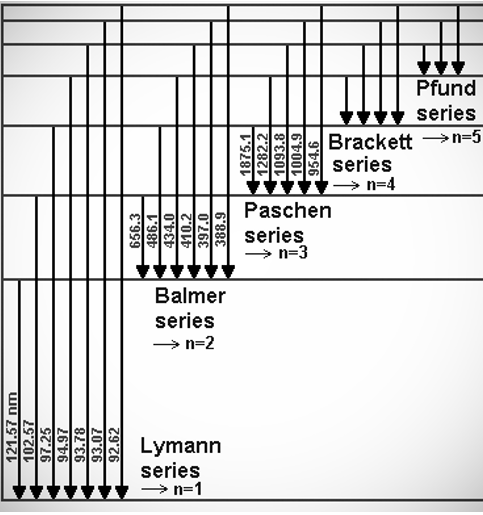
\includegraphics[width=5cm]{28-10.25(serie_idrogeno).png}
    \label{fig:serie_idrogeno}
  \end{figure}
\end{minipage}
\begin{minipage}{0.65\textwidth}
  \vspace{0.4cm}La figura accanto prende il nome di diagramma di Grotrian, in cui sono rappresentate tutte le possibili transizioni. Queste righe, se osservate, possono portare a conclusioni sulle condizioni della materia.

  Noi distinguiamo tutte le transizioni sul livello $n=1$ come \textbf{serie di Lyman} (sono nell'UV, la più esterna è a $120$ nm ed è in pieno UV, le altre sono a $\lambda$ ancora più brevi, quindi non sono visibili). Abbiamo poi la \textbf{serie di Balmer}, transizioni sul livello $n=2$ che sono visibili. Andando avanti osserviamo la \textbf{serie di Paschen} (queste sono nell'infrarosso).
\end{minipage}

\vspace{0.2cm}Sulla base del modello dell'atomo, si è dedotto che le righe spettrali sono dovute alle transizioni legato-legato, il continuo è dovuto alle transizioni libero-legato e a quelle libero-libero. Tale interpretazione si basa sulla \textit{fotoionizzazione}, cioè alla possibilità di estrarre un elettrone dall'atomo, trasferendo l'energia del fotone al sistema. Infatti abbiamo visto che ci sono transizioni con lunghezze d'onda ben precise (le varie serie), però c'è anche la possibilità di ionizzare. Noi possiamo misurare le energie di ionizzazione, le quali cambiano con l'elemento.

Concentriamoci sulle energie di prima ionizzazione. L'idrogeno richiede $13.6$ eV, l'elio $25$ eV, quando si va nei metalli questa energia diventa molto piccola. Questo significa che tutti i fotoni con un'energia maggiore di $13.6$ eV possono strappare un elettrone all'atomo di idrogeno, tutti i fotoni con un'energia maggiore di $5$ eV possono ionizzare il litio e così via.

\begin{figure}[H]
  \centering
  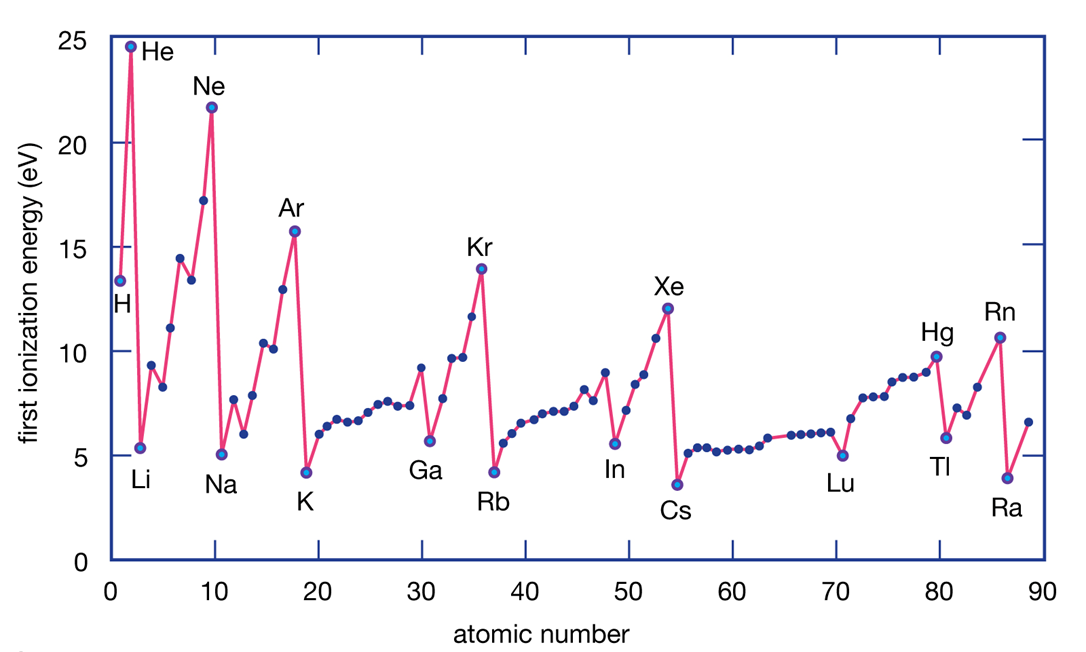
\includegraphics[width=9cm]{immagini/potenziale_ionizzazione.png}
  %\caption{Energie di prima ionizzazione di alcuni metalli}
\end{figure}

Vediamo come si potrebbe inserire questo primo concetto di ionizzazione nel trasporto radiativo. Quello che succede è che non basta che un fotone abbia l'energia sufficiente (questo è il prerequisito affinché ci sia la ionizzazione), ma poi la probabilità cambia con la lunghezza d'onda del fotone.

La ionizzazione di un atomo di idrogeno ha una probabilità di accadere, e questa probabilità viene definita come coefficiente di assorbimento:

$$\alpha_{bf}(\lambda,n)=\frac{\alpha_0 g_{bf} \lambda^3}{n^5}$$

dove $n$ è il livello di energia, quindi non è la stessa per tutti.

Il coefficiente di estinzione nasce dalla sommatoria sui vari stati e dal numero di atomi che hanno un elettrone in quello stato.

$${\chi_{\lambda}}(H_{bf})=\sum_{n_0}^{\infty} {\alpha_{bf}}({\lambda},n)\frac{N_n}{N}$$

%Qual è la probabilità che un gas di idrogeno possa assorbire dal campo di radiazione? La probabilità è legata alla distribuzione degli elettroni nei livelli orbitali.

Graficando questa quantità si ottiene:
    
\begin{figure}[H]
  \centering
  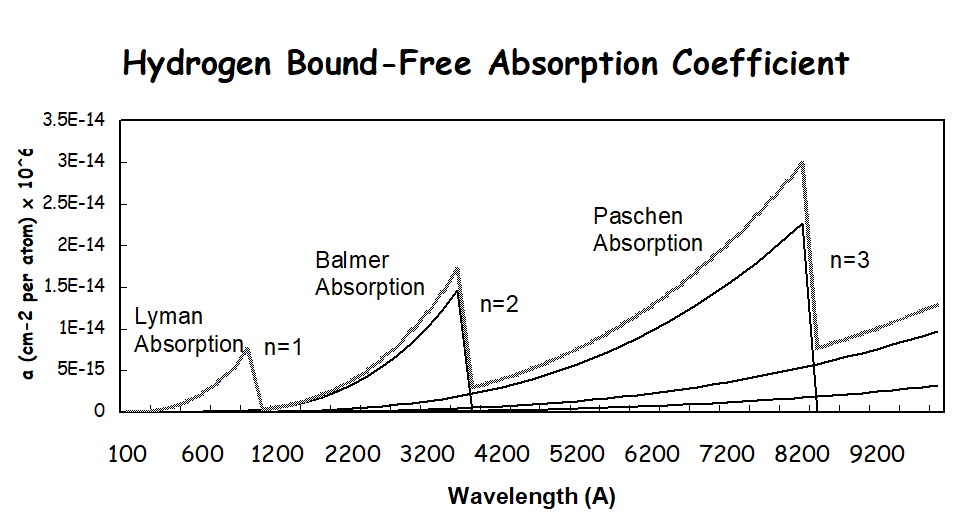
\includegraphics[width=10cm]{immagini/coefficiente_assorbimento_legato_libero_idrogeno.png}
  %\caption{Coefficiente di assorbimento per l'idrogeno}
  \label{fig: coefficiente di assorbimento }
\end{figure}

dove la parte in grigio rappresenta la somma dei termini; l'andamento in nero invece rappresenta il contributo dei vari livelli. Quindi, se è vero che il responsabile dell'estinzione è l'interazione atomica tra radiazione e idrogeno, questo si dovrebbe ritrovare negli spettri. Ed effettivamente accade.

\begin{figure}[H]
  \centering
  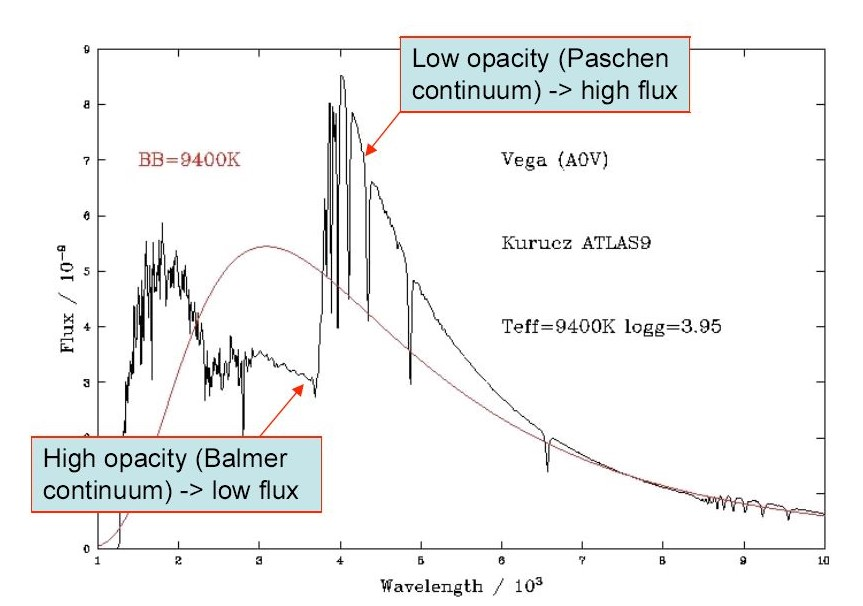
\includegraphics[width=10cm]{spettro_stella.jpg}
\end{figure}

Questo è il tipico spettro di una stella con l'energia in funzione della lunghezza d'onda. Quello che noi vediamo nelle stelle è il reciproco della probabilità di ionizzazione.

Il salto che osserviamo, che si chiama Balmer jump, è stata considerata la prova sperimentale della fotoionizzazione.

\vspace{0.2cm}Come si spiega il fatto che esistano stelle il cui Balmer jump ha dimensione diversa?

Il fatto che non esista in alcune stelle è considerata una prova che la temperatura della stella è così alta che non esiste idrogeno neutro. Se non esiste l'idrogeno neutro, non si possono fermare fotoni di lunghezza d'onda ultravioletta e quindi si avrà un certo andamento. Poi ci saranno delle stelle in cui il secondo livello dell'idrogeno è molto popolato e quindi potrà assorbire molti fotoni; poi ci sono delle condizioni per stelle più fredde (che noi vediamo rosse) che non hanno elettroni nel livello 2, ma ce li hanno tutti nel livello 1. Quindi, avendo tutti gli elettroni nel livello 1, potranno solo trattenere i fotoni da 1200 Å (quelli di alta energia). Tale fatto è spiegato matematicamente dall'equazione di Saha:

$$\frac{n_{i+1}}{n_{i}} n_{e}= \frac{2}{\Lambda^3} \frac{g_{i+1}}{g_{i}} e^{-\frac{(\epsilon_{i+1} - \epsilon_i)}{k_BT}}$$

dove

\begin{itemize}
  \item $\displaystyle \Lambda=\sqrt{\frac{h^2}{2 \pi m_3 k_B T}}$;
  \item $g_i$ è il peso statistico o molteplicità dei livelli, rappresenta il numero di modi in cui possono essere sistemati le particelle nei vari livelli;
  \item $\epsilon_i$ è l'energia necessaria per rimuovere $i$ elettroni da un atomo neutro;
  \item $n_e$ è la densità elettronica.
\end{itemize}

Infatti, dato un gas, i suoi atomi si possono trovare ad un diverso stato di ionizzazione, e tale equazione ci dice che, dati due stati di ionizzazione successivi $n_{i+1}$ e $n_i$ (ad esempio idrogeno neutro e idrogeno ionizzato) il rapporto tra le due quantità dipende innanzitutto dalla densità elettronica (e questo è intuitivo, perché se dobbiamo ionizzare si devono avere elettroni liberi pronti per essere ricatturati: all'equilibrio la ionizzazione è ostacolata dai tanti elettroni liberi), dalla temperatura del gas e dall'energia di ionizzazione.

Riportando il numero di atomi ionizzati in funzione della temperatura, l'equazione assume una forma di questo tipo:
  
\begin{figure}[H]
   \centering
   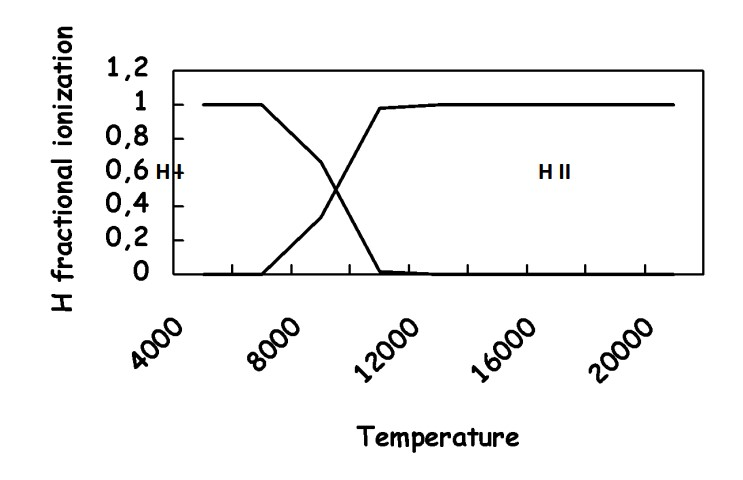
\includegraphics[width=10cm]{Saha_equation.jpg}
   %\caption{Equazione di Saha}
\end{figure}

Se abbiamo un gas e cominciamo a scaldarlo, osserviamo che a temperature dell'ordine di $4000$ K il gas è tutto legato (non è detto che tutti gli elettroni siano nel livello fondamentale, però tutti gli elettroni sono legati). Quando andiamo a temperature di $20000$ K tutti gli elettroni sono staccati dai nuclei, il gas è quindi tutto ionizzato; a tali temperature il coefficiente di opacità dovuto alla ionizzazione dell'idrogeno non è più importante, in quanto non ci sono più elettroni che possono assorbire quella radiazione. Abbiamo poi la regione di mezzo in cui parte della radiazione è assorbita e parte no.

\textbf{questa frase l'ho messa io quindi sono molto dubbioso}L'equazione di Saha può essere scritta, considerando il il numero di atomi in un livello rispetto al totale, come

$$\frac{N_n}{N}=\frac{g_n}{u_0(T)} e^{-\frac{\chi}{kT}}$$

dove $u_0(t)$ è la funzione di partizione e si usata come notazione infelice $\chi$ per indicare l'energia di ionizzazione. Il coefficiente di assorbimento allora diventa

\begin{equation*}
  \chi(\text{H}_{bf})= \alpha_n \sum_{n_0}^{\infty} \frac{\lambda^3}{n^3} g_{bf} e^{-\frac{\chi}{kT}}
\end{equation*}
 
Qual è quindi il coefficiente di estinzione dovuto all'idrogeno per quanto riguarda le possibili transizioni legato-libero? Questo coefficiente nasce dalla probabilità che un atomo con un elettrone in un livello possa assorbire. Se un atomo di idrogeno ha un certo elettrone in un certo livello, c'è una probabilità di interazione. A questo punto l'estinzione è data dal numero di atomi che sono in quel livello. Però dobbiamo anche sapere quanti sono gli atomi di idrogeno non ionizzati. Supponiamo di vedere scomparire 100 fotoni dal mio campo di radiazione, se vogliamo risalire alla vera quantità di idrogeno dovrò chiedermi qual è la probabilità che un atomo venga ionizzato.

Parliamo di probabilità, le probabilità sono ovviamente prodotti di probabilità.

Il coefficiente di estinzione è la probabilità che un fotone di una certa lunghezza d'onda venga assorbito. Allora noi ci dobbiamo chiedere quali sono gli ingredienti per questo assorbimento.

Innanzitutto deve esistere l'atomo nello stato in cui può assorbire (nel caso specifico deve esistere l'atomo neutro di idrogeno, che è una probabilità che, dato l'idrogeno, questo sia allo stato neutro). Ammesso che abbiamo un atomo neutro, la probabilità che un fotone venga assorbito ad una lunghezza d'onda è legata al livello energetico in cui si trova l'elettrone. Quindi, per sapere quanti fotoni sono stati assorbiti dobbiamo sapere quanti sono gli atomi di idrogeno neutro che hanno elettroni nel livello $n$.

Dobbiamo quindi sapere qual è la distribuzione degli elettroni tra i livelli, quando l'ho scoperta posso moltiplicare ciascuno di questi per il coefficiente di assorbimento. Quindi un coefficiente di estinzione, per quanto riguarda le transizioni legato-libero, si presenta come una sommatoria tra tutti i casi che possono assorbire quella lunghezza d'onda.

Se lo volessimo fare numericamente non sarebbe difficile.
Qui di nascosto c'è la temperatura dello strato. Supponiamo che questo sia il Sole e supponiamo di guardare la luce dall'alto e di disegnare i vari stati (tanti strati): voglio sapere qual è la temperatura per ogni strato. Posso imporre come una condizione di equilibrio, come sulla Terra? Perfetto, qui ho un'idea di temperatura. Con questa temperatura mi devo chiedere quanti sono gli atomi di idrogeno neutri, quanti sono gli atomi di idrogeno ionizzati (e quindi quanti sono i fotoni). Una volta che l'ho calcolato mi devo chiedere "ma qui come sono distribuiti tra i livelli"? Quando mi sono dato una risposta, posso moltiplicare questi numeri per il coefficiente di assorbimento e sapere quanti fotoni vengono bloccati "qui", poi questi fotoni li passo al livello successivo e mi chiedo quanti fotoni possono essere assorbiti qua, e così via.
Questo diventa nell'equazione del trasporto, la costruzione di questo $\tau$ che è dato dalla somma di $\chi$ per numero di particelle per $ds$.